
%Include the complete description of the methods used in your research here. %\\

In this chapter, a detailed account has been presented of the research design, data collection and analysis, and the steps taken to ensure the validity and reliability of the study. The aim of this chapter is to provide readers with a clear understanding of the research methodology and the rationale behind the chosen approach in respect to the deep learning models chosen and related work. The following sections will detail the process of classifying fish species using deep learning, including the data collection and pre-processing, model architecture, training and evaluation, and the steps taken to ensure the accuracy and robustness of the results. 

\section{Data Collection}

\noindent As discussed earlier, the thesis aims at classification of fish species which are found in freshwater like rivers and lakes. Collecting data for species which are in a river is generally a very difficult task considering the water flow, depth of stream and other natural conditions such as growth of algae, weed, lighting conditions etc. The industrial partner developed an autonomous camera that can be positioned underwater in Norway's rivers and fjords specifically for this use. In order to reduce the stress on the users, the system combines a combination of effective and powerful machine vision algorithms. The hardware is able to withstand adverse situations and lengthy service intervals because it is durable, light, and compact. The camera system has an embedded local computer with AI-specific accelerator which has the capacity to process over 1 million images per day. The AI accelerator by Coral features on-device inferencing capabilities that enable the development of productive, discreet, quick, and offline products. The fish detection system that is installed locally on the system allows the accelerator to record videos when there is a fish detection by the algorithm. These videos are further processed into frames which results in images of the fish. No specific species is targeted during the detetcion of the fish by the algorithm. Therefore a large number of fish images is collected at the central repository. The images are further identified and approved by the specialists in this field and labelled correctly as fish or no-fish. Since there is a large data available for fish, it is possible to further label the fish according to the specie they belong to using labelbox. Labelbox is platform where teams can collaboratively label data for machine learning applications for collaborative data labeling. It offers a web-based interface for labeling text, polygonal segmentation masks, object bounding boxes, and pictures, videos, and other sorts of data. Once the data is labeled, it can be used as dataset for various machine learning applications such as object detection, object classification etc. For the purpose of this project, the species that was identified was trout. Within the trout specie, there are two categories of interest for fish farmers and aquaculture which are trout and mature trout. Mature trout are simply adult trout that have reached sexual maturity and are capable of reproducing. The following is the distribution of data that has been provided for the project-

\begin{table}[ht!]
\centering
    \begin{tabular}{ m{3cm} m{5cm} m{3cm} } 
    \toprule
    \toprule
    \textbf{Label} & \textbf{Label Count} & \textbf{Distribution} \\
    \midrule
    trout    & 25270    & 84\%                      \\[1.3ex]
    mature trout    & 4696    &  15\%                      \\[1.3ex]
    damaged    & 58    & <1\%                       \\[1.3ex]
    \bottomrule
    \end{tabular}
\caption[Data distribution]{Data distribution}
\label{table:data_distribution}
\end{table}

Since the aim of the project was to build a classifier for the classification of trout and mature trout, and considering the number of images in 'damaged' category is very low, only the trout and mature trout categories were chosen to proceed with. The total labelled images that are available for the project were 29966 images. The data is not balanced and this has to be taken into consideration when working with any deep learning model for classification. It is important to note that all the images are taken in a same environment with respect to light and background conditions. These images can contain multiple or single fish which can belong to mature or trout category. Following are a couple of sample images that are from the labelled dataset-
\begin{figure}[ht!]
  \centering
  \begin{minipage}[b]{0.4\textwidth}
    \centering
    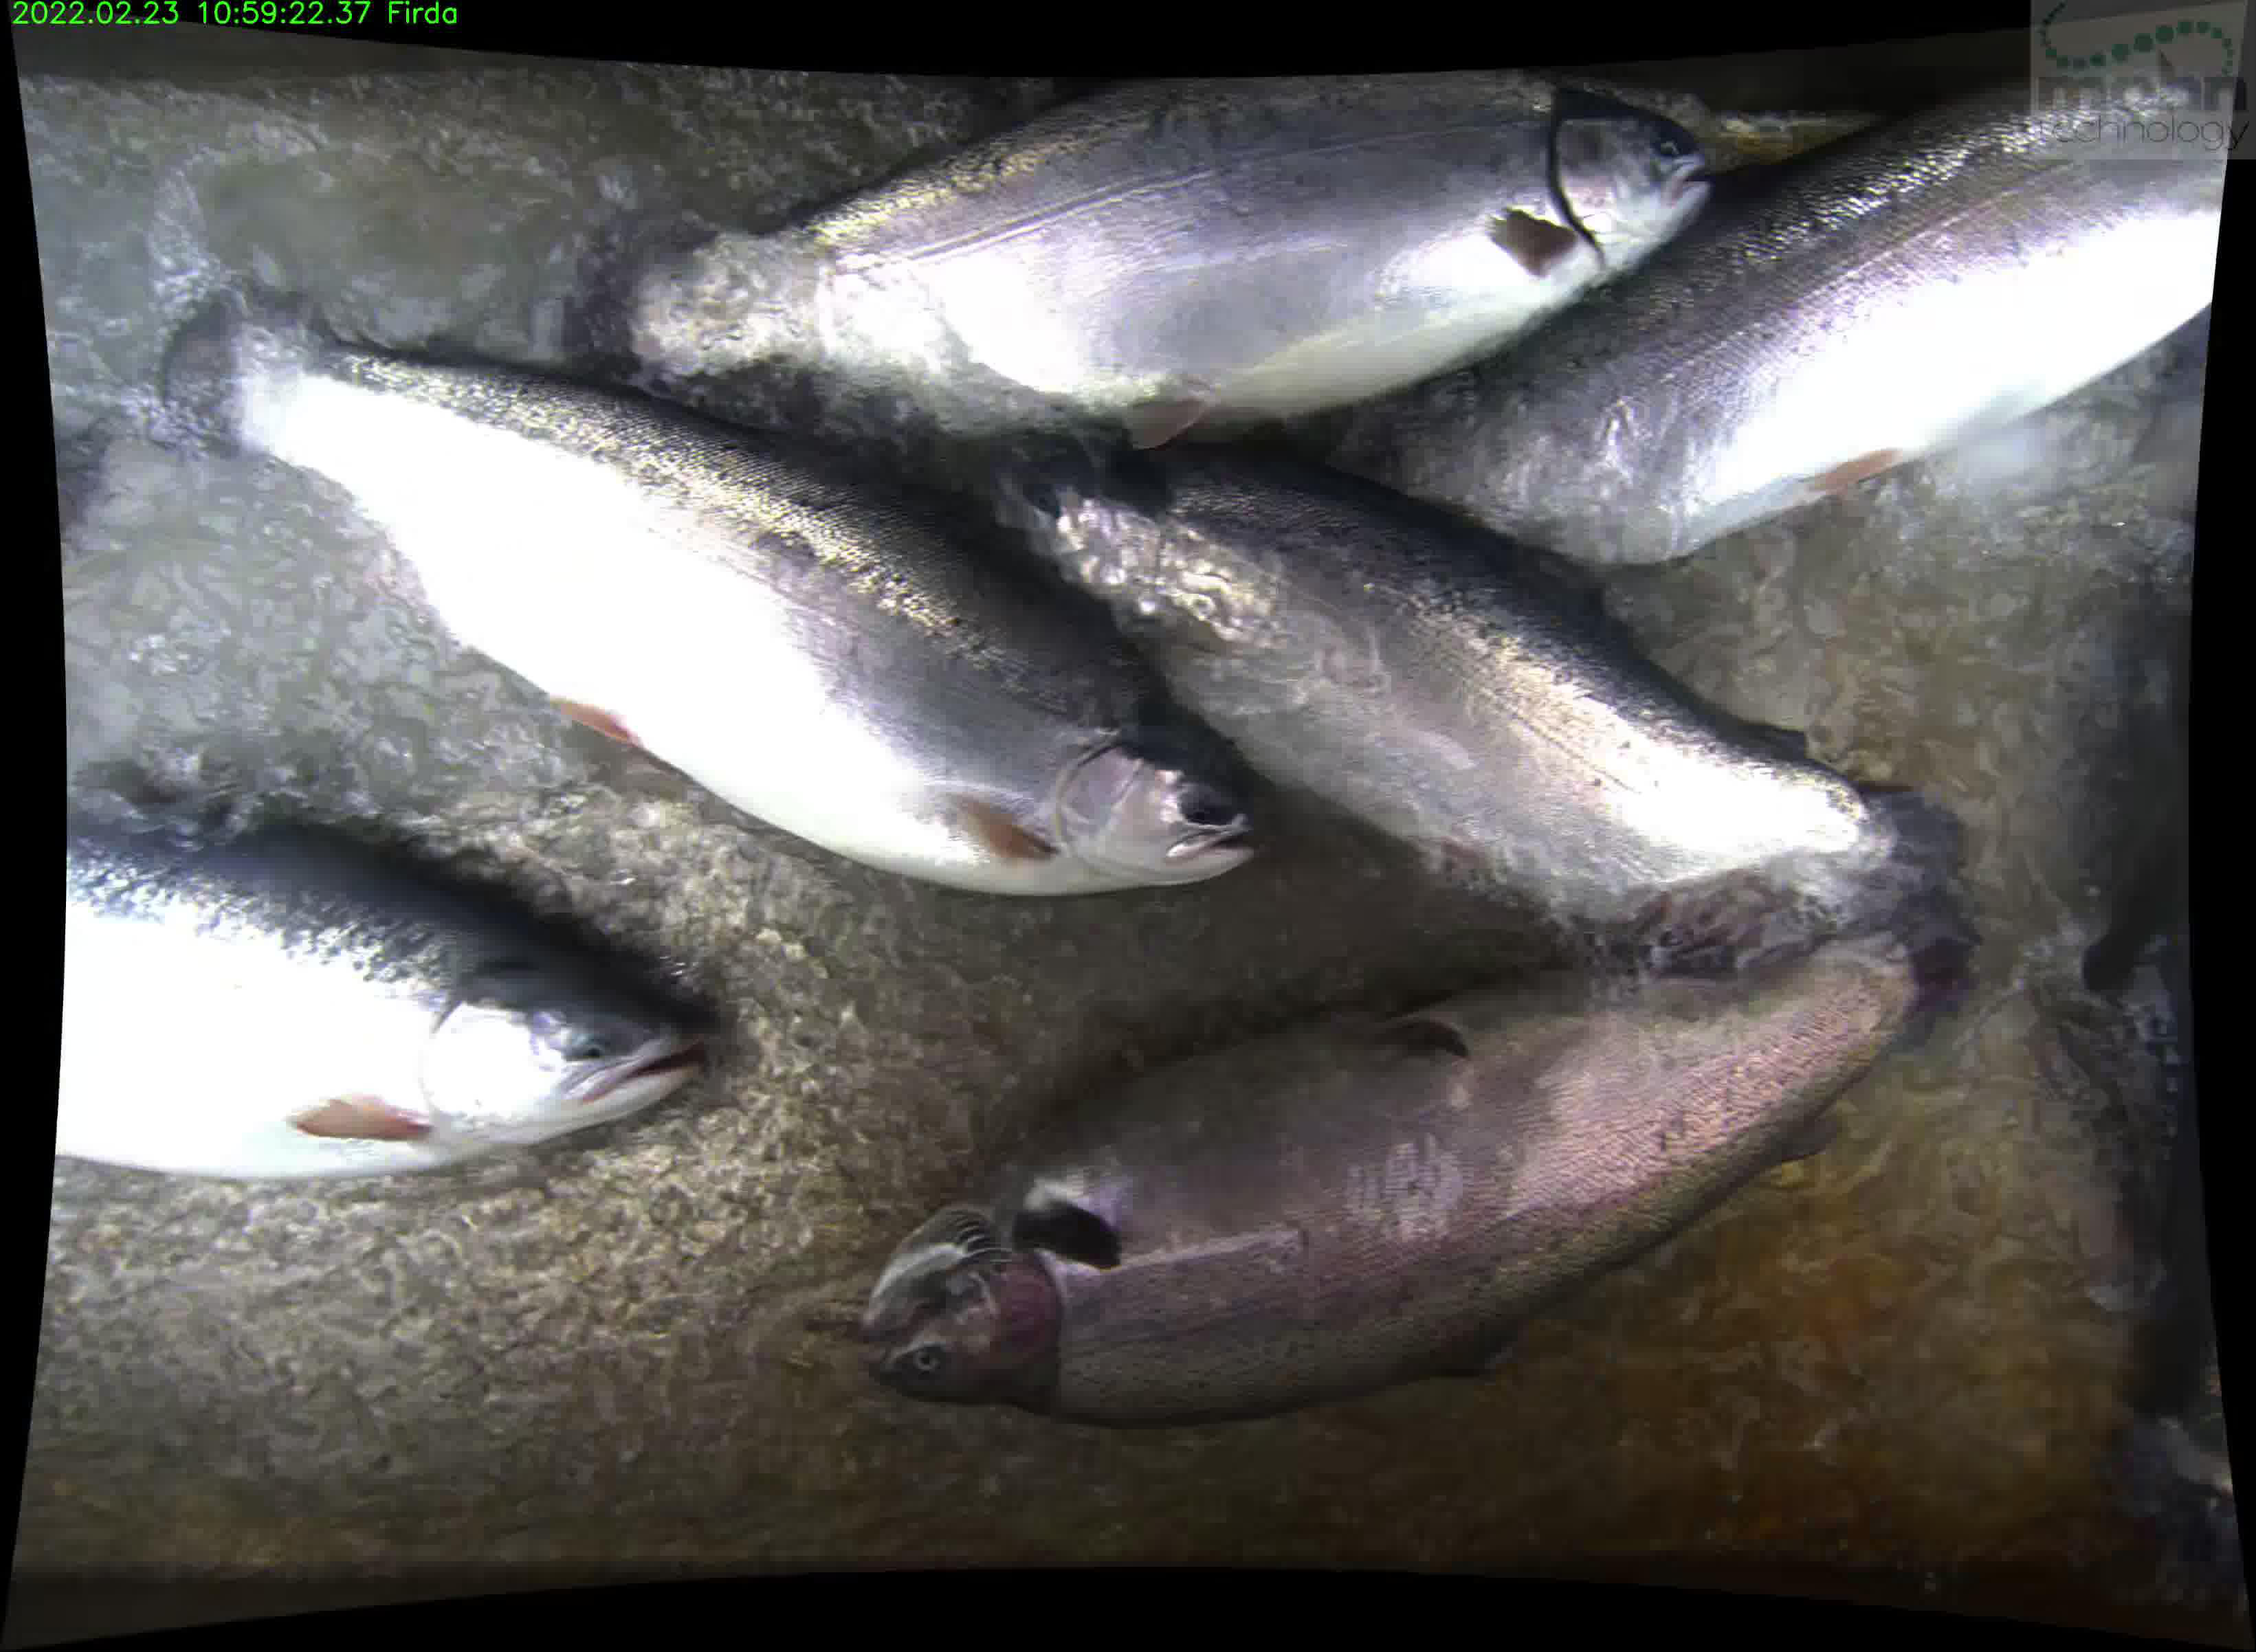
\includegraphics[width=\textwidth]{Figures/img_1.jpg}
    \caption{Dataset image 1}
    \label{fig:image1}
  \end{minipage}
  \hfill
  \begin{minipage}[b]{0.4\textwidth}
    \centering
    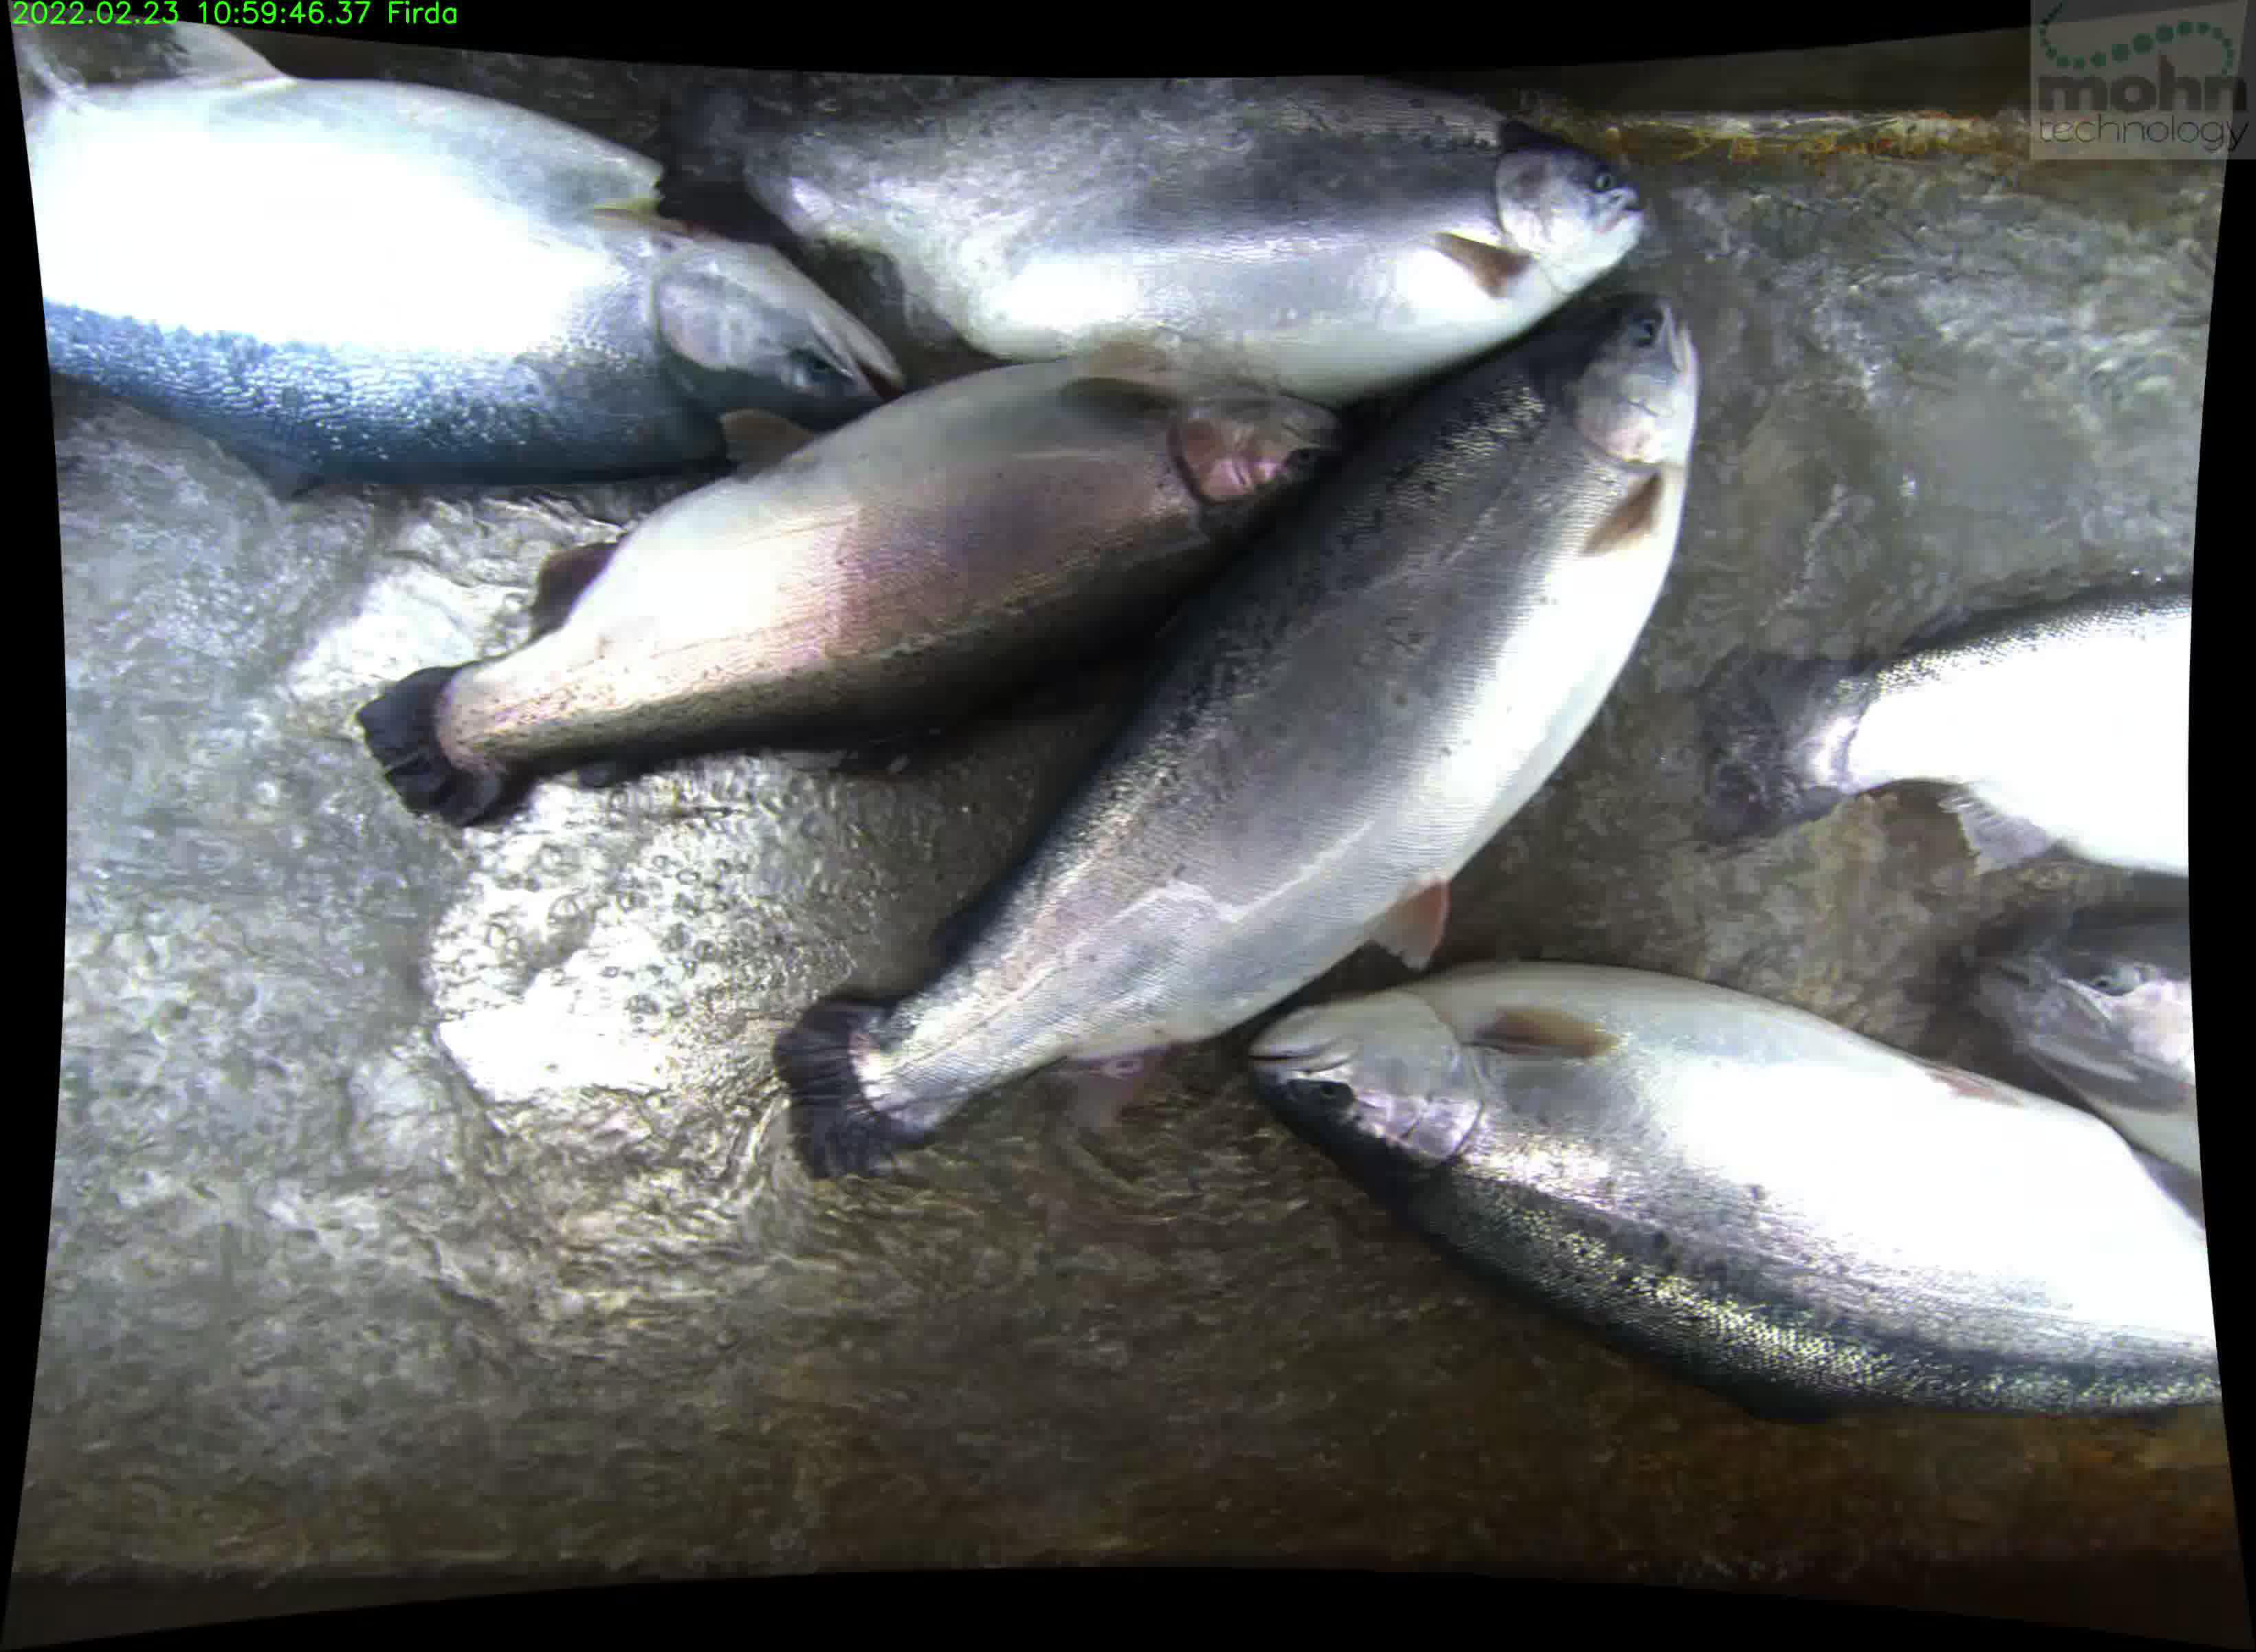
\includegraphics[width=\textwidth]{Figures/image_2.jpg}
    \caption{Dataset image 2}
    \label{fig:image2}
  \end{minipage}
\end{figure}

The sections further will explain in detail how this data has been processed and prepared to be used in training models for the classification of trout and mature trout.

\section{Data Pre-processing}

The data that is available for 2 label categories trout and mature trout (which is labelled as mature) are images with single or multiple fish in the frame. The following images are a sample of what the images with detection frame look like: 
\begin{figure}[H]
  \centering
  \begin{minipage}[b]{0.45\textwidth}
    \centering
    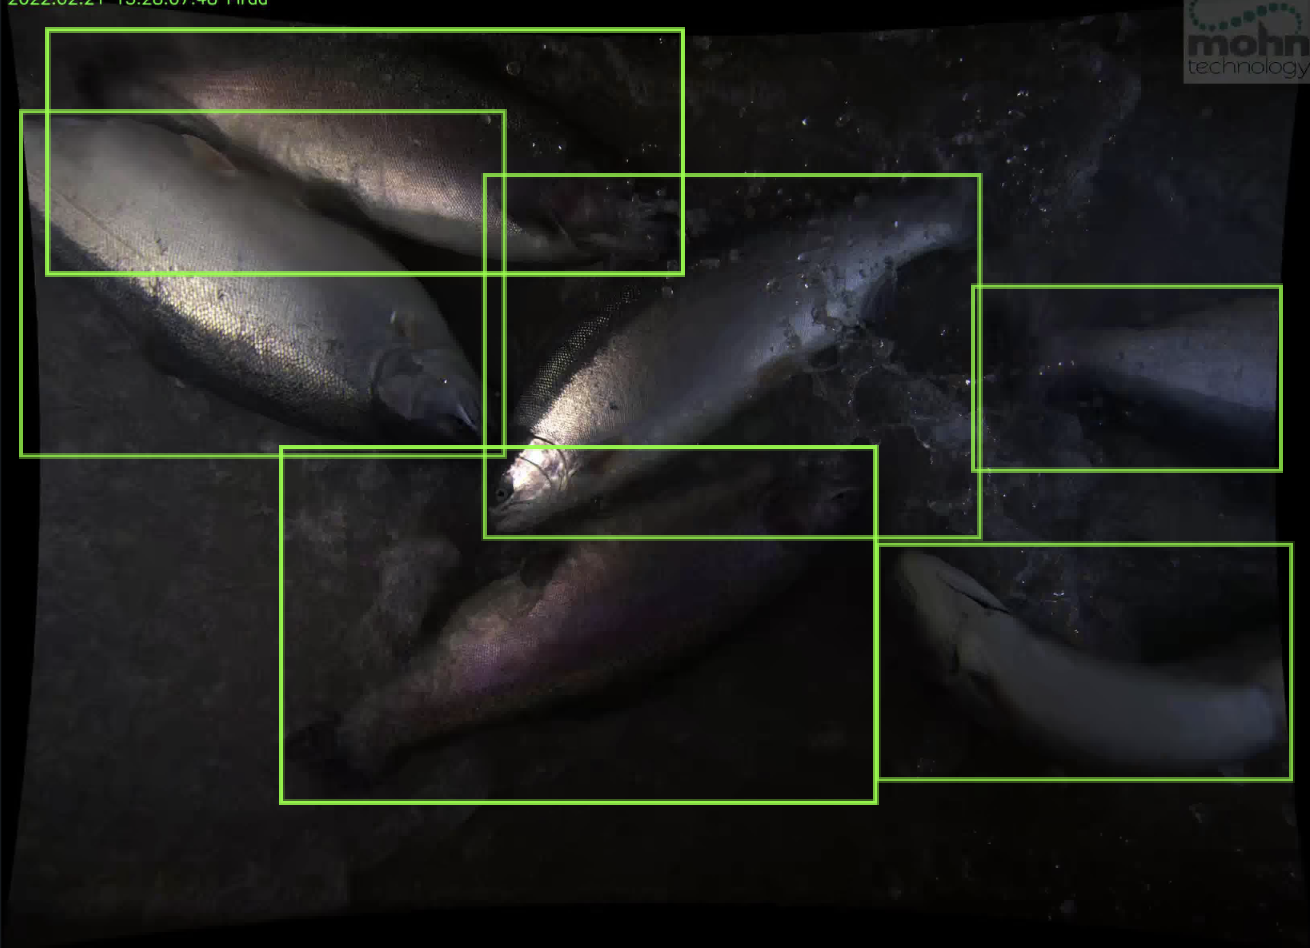
\includegraphics[width=\textwidth]{Figures/detection1.png}
    \caption{Detection image 1}
    \label{fig:detection1}
  \end{minipage}
  \hfill
  \begin{minipage}[b]{0.45\textwidth}
    \centering
    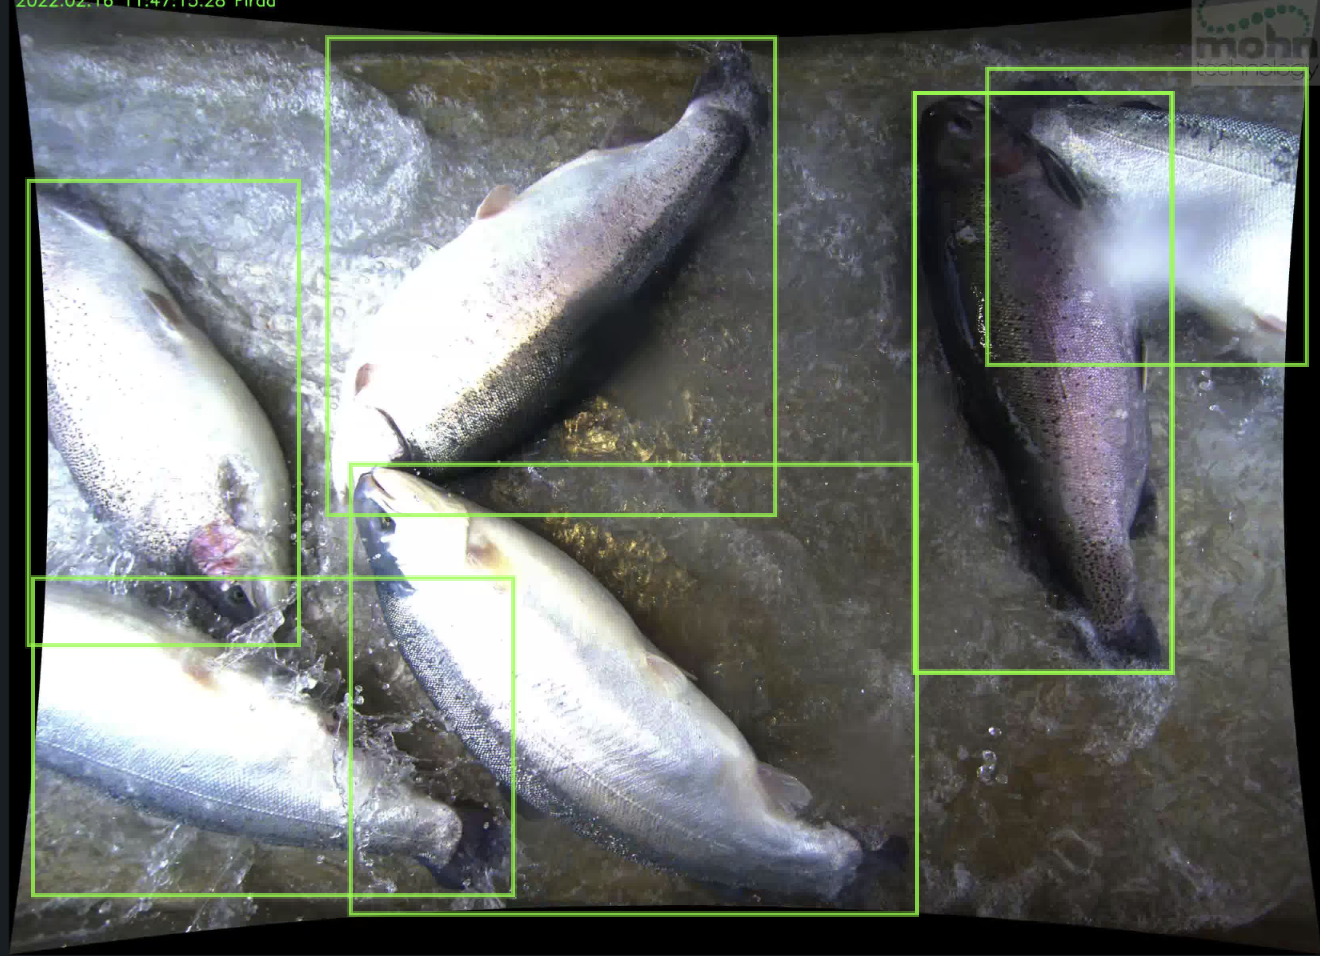
\includegraphics[width=\textwidth]{Figures/detection2.png}
    \caption{Detection image 2}
    \label{fig:detection2}
  \end{minipage}
  \begin{minipage}[b]{0.45\textwidth}
    \centering
    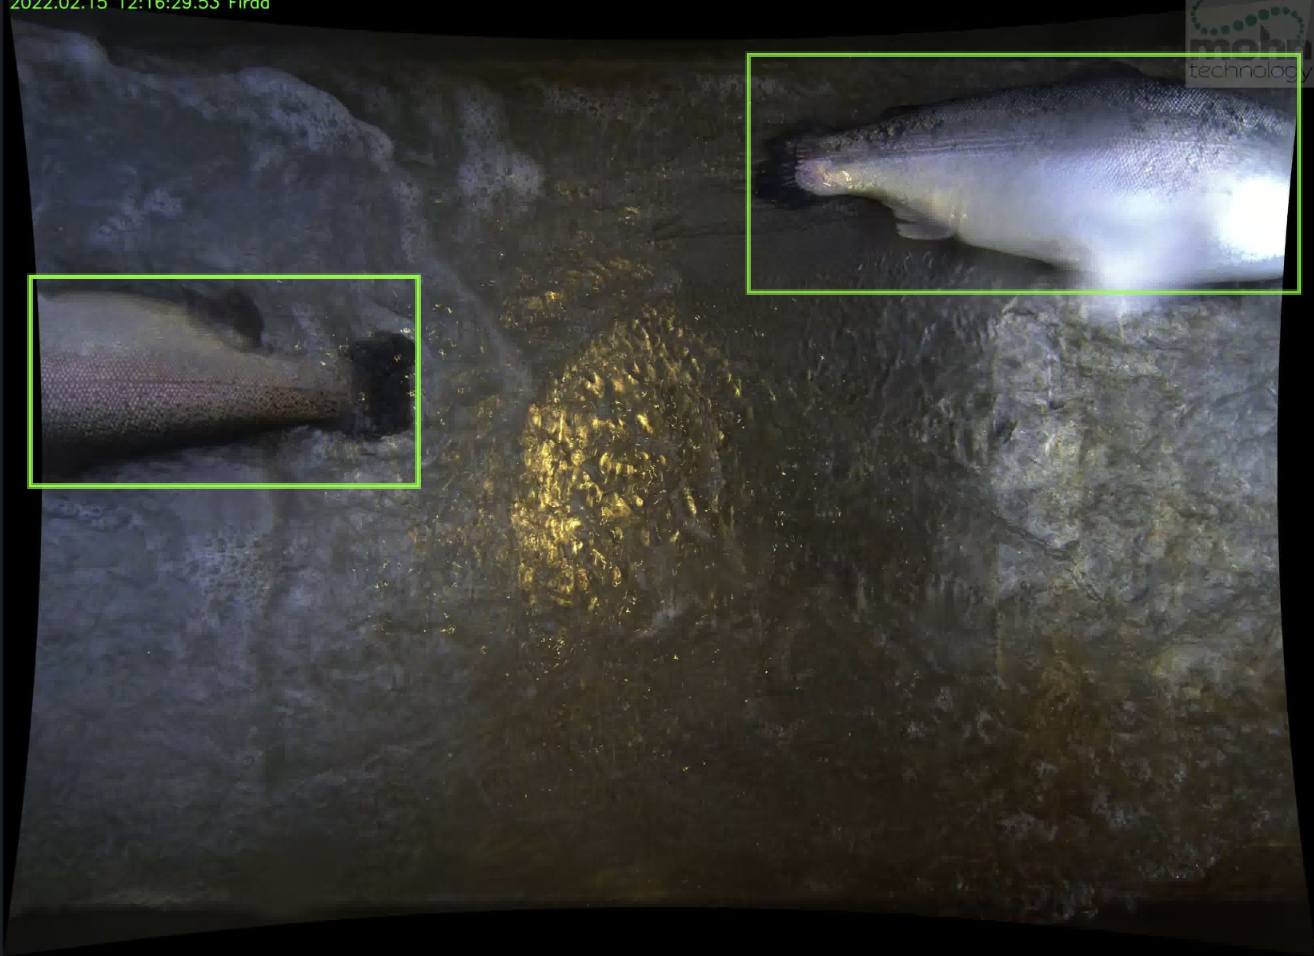
\includegraphics[width=\textwidth]{Figures/detection3.png}
    \caption{Detection image 3}
    \label{fig:detection3}
  \end{minipage}
  \hfill
  \begin{minipage}[b]{0.45\textwidth}
    \centering
    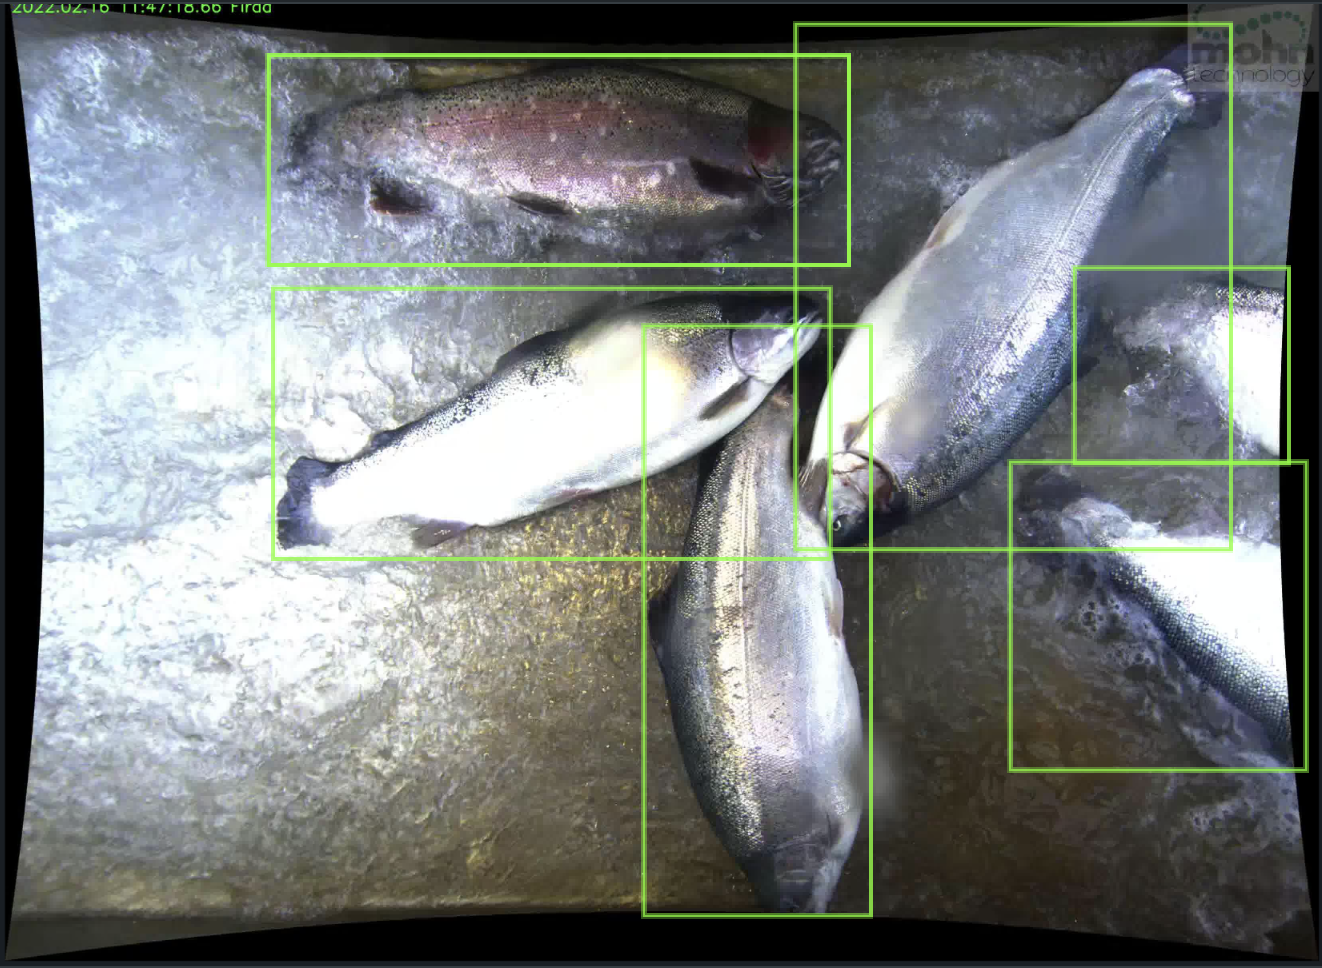
\includegraphics[width=\textwidth]{Figures/detection4.png}
    \caption{Detection image 4}
    \label{fig:detection4}
  \end{minipage}
\end{figure}
The data which was available at labelbox central repository, was downloaded using APIs support. Using the project id which is related to the dataset, all the images that are labelled are downloaded. Each image also has the associated annotation files in pascal voc format. These files contain some relevant information about the related images such as bounding box coordinates for the detection and the associated class label. In this case, the labels we are talking about are \textbf{trout} and \textbf{mature}. Since we are looking forward to a classification algorithm, it is important to get the data sorted based on the class so that it can be prepared for training, validation and test sets. To prepare the dataset, a python script was written to loop through the pascal voc file which has the respective filename for the image, loop through the labels in each image and create a cut out of each detection. Each detection is then saved to the respective directories which are called trout and mature. At the end, we get 25270 images of trout and 4696 images of mature category. With a digital cut out of the target class from the detection images, we get a more precise image of the class that we want to train the algorithm with. In this way, the extra 'noise' in the original images such as background and the empty spots can be ignored and we end up with a more concrete dataset which has only the images that are relevant to the class. \\

Following are sample of images from the trout class:
\begin{figure}[H]
  \centering
  \begin{minipage}[b]{0.4\textwidth}
    \centering
    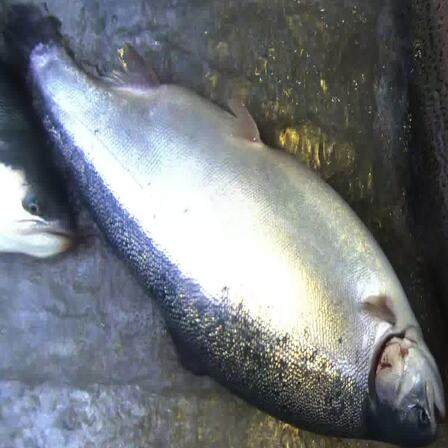
\includegraphics[width=3.5in, height=2in, keepaspectratio]{Figures/trout1.jpg}
    \caption{Trout image 1}
    \label{fig:trout1}
  \end{minipage}
  \hfill
  \begin{minipage}[b]{0.4\textwidth}
    \centering
    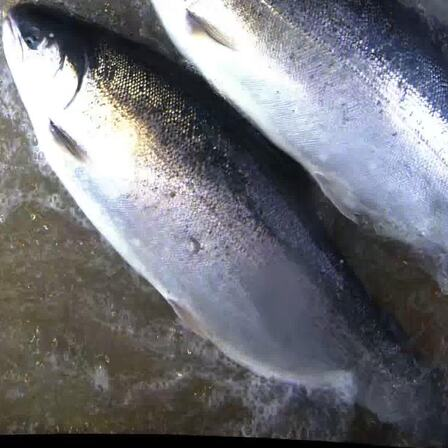
\includegraphics[width=3.5in, height=2in, keepaspectratio]{Figures/trout2.jpg}
    \caption{Trout image 2}
    \label{fig:trout2}
  \end{minipage}
\end{figure}

\\  Following are sample of images from the mature class:

\begin{figure}[H]
  \centering
  \begin{minipage}[b]{0.4\textwidth}
    \centering
    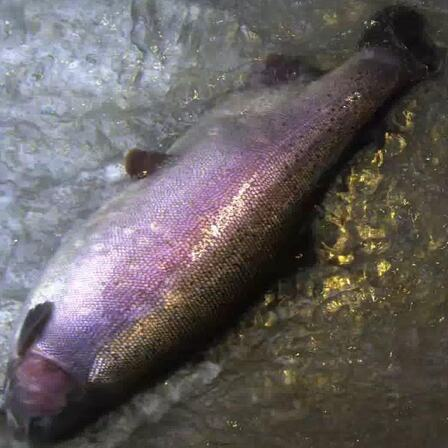
\includegraphics[width=3.5in, height=2in, keepaspectratio]{Figures/mature1.jpg}
    \caption{Mature image 1}
    \label{fig:mature1}
  \end{minipage}
  \hfill
  \begin{minipage}[b]{0.4\textwidth}
    \centering
    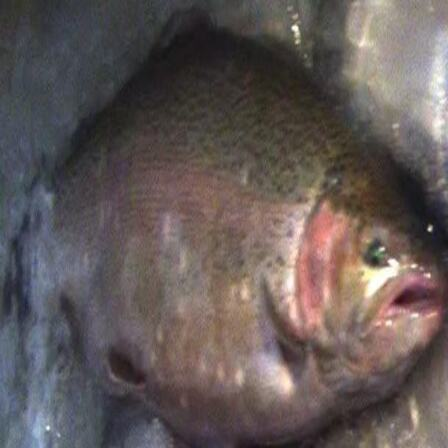
\includegraphics[width=3.5in, height=2in, keepaspectratio]{Figures/mature2.jpg}
    \caption{Mature image 2}
    \label{fig:mature2}
  \end{minipage}
\end{figure}

The two categories of fish have quite a lot of similarities in their size and dimensions as can also be seen in the images. The mature category has a slight red tinge on the body. This may or may not be very significant differentiating factor and the lighting condition in the images can also affect how easy or difficult it is manually to classify an image as mature or not. \\ 

Following are sample of images from the mature category which has quite a lot of variation in the color shade as compared to trout category:

\begin{figure}[H]
  \centering
  \begin{minipage}[b]{0.4\textwidth}
    \centering
    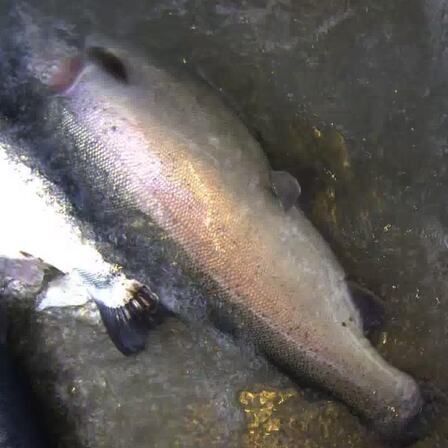
\includegraphics[width=3.5in, height=2in, keepaspectratio]{Figures/lightshademature.jpg}
    \caption{Light shade mature}
    \label{fig:maturelight}
  \end{minipage}
  \hfill
  \begin{minipage}[b]{0.4\textwidth}
    \centering
    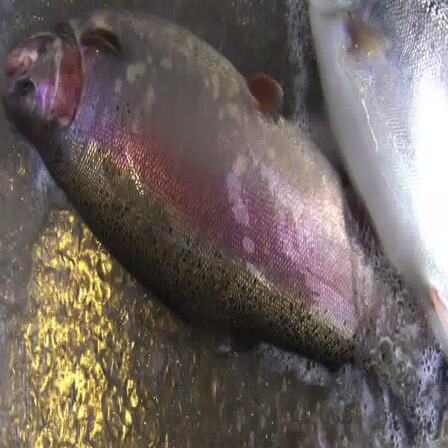
\includegraphics[width=3.5in, height=2in, keepaspectratio]{Figures/darkshademature.jpg}
    \caption{Darker shade mature}
    \label{fig:maturedark}
  \end{minipage}
\end{figure}

Since the two category of fish in discussion are not very different from each other, some types of image pre-processing techniques such as gray scaling of images (which will convert the images to gray scale), Gaussian blurring  (which is used to blur the image and reduce noise) and histogram equalization because these can alter the color balance of the image.
\\
When the data is loaded as a dataset in the code, it also undergoes several pre-processing. The \textbf{'tf.keras.preprocessing.image\_dataset\_from\_directory'} function creates a \textbf{'tf.data.Dataset'} object from image files stored in a directory. This function performs several pre-processing steps on the images, including:
\begin{itemize}
    \item Resizing the images to the specified \textbf{image\_size} which is (224,224) and is the required input image size for the compatible models \url{https://coral.ai/models/image-classification/} \cite{coralModelsImage}. 
    \item Batching the images into batches of the specified \textbf{batch\_size}
    \item Shuffling the batches of images randomly
    \item The \textbf{seed} parameter in the function sets the random seed for shuffling the batches of images.
\end{itemize}
Once the data is loaded into the memory, it is also scaled from the range of [0, 255] to [0, 1]. This is done so that the input data that is normalized to a small range of values, typically [0, 1] or [-1, 1].
\\
These pre-processing steps are performed to prepare the data for training a model. Resizing the images ensures that they all have the same dimensions, which is necessary for feeding them into a neural network. Converting the images to floating-point tensors and scaling their pixel values to the range [0, 1] is also necessary for compatibility with neural network models. Batching the images into smaller groups allows the model to process them more efficiently during training. Shuffling the batches randomly helps to ensure that the model sees a diverse set of images during each epoch of training. In the end, applying a lambda function using the \textbf{'map'} method, the resulting \textbf{'tf.data.Dataset'} object contains the scaled images and their corresponding labels, which can be used for training the model.

The next step in the pre-processing is preparing the dataset for the training of the model. The splitting of the data into training, validation, and test sets is done using the \textbf{tf.data.Dataset} API in TensorFlow. For this, the length of the entire dataset data is used to compute the number of samples to allocate to each set. The training set gets 70\% of the samples, the validation set gets 20\% of the samples, and the test set gets the remaining 10\% of the samples. The \textbf{take} method is used to extract the first \textbf{train\_size} number of samples from the dataset data, which become the training set. The \textbf{skip} method is used to skip over the training samples, and then the \textbf{take} method is used again to extract the next \textbf{val\_size} number of samples from the remaining data, which become the validation set. Finally, the \textbf{skip} and \textbf{take} methods are used again to extract the remaining \textbf{test\_size} number of samples, which become the test set. The training set is used to train the model, while the validation set is used to evaluate the performance of the model during training and make decisions about hyperparameters such as learning rate, number of epochs, etc. This also helps in preventing overfitting and improve the generalization of the model.
 

\section{Data Augmentation}

As discussed in the section above, there is a high imbalance in the number of images for trout and mature labels. The images for trout category are almost 6 times the images for mature category. There should be a balance in the dataset so that the model is not biased towards the majority class and poorly on the minority class. The performance of the model will be affected and which is why it is important to have data augmentation because this has been one of the proven ways to improve accuracy of models dealing with classification tasks \cite{perez2017effectiveness}. 

For the project, two methods were used to balance the data set. One of the way was where the trout class which has 25570 images,  was selected and using a python script, random 5000 files were selected and moved to a new directory. The results from this distribution of data will be discussed in the further sections. The other method was to apply data augmentation on the 4696 images that are available in the mature class, and increase the data for this class to 6 times and come closer to the count for trout class. To artificially increase the amount of training data available by generating modified versions of the original data, the Keras \textbf{ImageDataGenerator} class was used. The different parameters defined to generate the images are:
\begin{itemize}
    \item \textbf{rotation\_range}: Specifies the range (in degrees) for random rotations of the image. For example, if rotation\_range=10, the image can be rotated randomly between -10 and 10 degrees.
    \item \textbf{width\_shift\_range}: Specifies the range (as a fraction of the total width) for horizontal shifts of the image.
    \item \textbf{height\_shift\_range}: Specifies the range (as a fraction of the total height) for vertical shifts of the image.
    \item \textbf{shear\_range}: Specifies the range (in degrees) for random shearing transformations of the image.
    \item \textbf{zoom\_range}: Specifies the range for random zooms of the image
    \item \textbf{horizontal\_flip}: Specifies whether to randomly flip images horizontally.
    \item \textbf{vertical\_flip}: Specifies whether to randomly flip images vertically.
    \item \textbf{fill\_mode}: Specifies how to fill in any new pixels created during the transformation. The 'nearest' mode is used, which means that the nearest pixel will be used to fill in the new pixel values.
\end{itemize}

The 'ImageDataGenerator' object is created with these parameters and the code uses the \textbf{flow} method \cite{tensorflowTfkeraspreprocessingimageImageDataGeneratorTensorFlow} of the 'ImageDataGenerator' object to generate batches of augmented data. The different parameters used here are:

\begin{itemize}
    \item \textbf{img}: This is the input image that will be augmented. It is a 3D NumPy array representing the image.
    \item \textbf{batch\_size}: This parameter specifies the number of images to be generated in each batch.
    \item \textbf{save\_prefix}: This parameter specifies a prefix to use when saving the generated images. The actual file names will be the prefix followed by an index number and the specified file format.
    \item \textbf{save\_format}: This parameter specifies the file format to use when saving the generated images which in this case is 'jpg'.
    \item \textbf{save\_to\_dir}: This parameter specifies the directory in which to save the generated images. If None (the default), the images will not be saved to disk and will only be generated in memory but for the project, the path has been specified to a directory so that the images can be saved on disk.
\end{itemize}

Using a python script, each image was passed through the 'flow' method to generate 5 augmented images from one single image. This way the data was increased artificially for the mature category. Following are the sample augmented images which are generated from a single base image:

%add images here for augmentation

Following is the distribution of data between the two classes before and after augmentation:

\begin{table}[ht!]
\centering
\begin{tabularx}{\textwidth}{@{} *5{X} @{}}
\toprule
\textbf{Label} & \textbf{Label count before} & \textbf{Label count after} & \textbf{Distribution before} & \textbf{Distribution after} \\
\midrule
    trout     & 25270 & 25270  & 84\%  & 50\%  \\[1.3ex]
    mature    &  4696 & 25612  & 16\%  & 50\%  \\[1.3ex]
    total     & 29966 & 50882  & 100\% & 100\% \\[1.3ex]
\bottomrule
\end{tabularx}
\caption{Data distribution before and after augmentation}
\label{table:data_augmentation}
\end{table}


\section{Model Architecture}

As discussed in the proposal earlier, the industry partner has expressed a preference to work with TensorFlow 2.0 \cite{tensorflowEffectiveTensorflow}, therefore the chosen models are the ones that are compatible with TensorFlow 2.0. A list of the models that are compatible with Coral Edge TPU at the time of writing this are as follows:

\begin{table}[ht!]
\centering
\begin{tabularx}{\textwidth}{@{} *3{X} @{}}
\toprule
\textbf{Model Name} & \textbf{Dataset} & \textbf{Input Size}\\
\midrule
    MobileNet V1     & ImageNet & 224x224x3   \\[1.3ex]
    MobileNet V2    &  ImageNet & 224x224x3  \\[1.3ex]
    MobileNet V3     & ImageNet & 224x224x3  \\[1.3ex]
    ResNet-50     &  ImageNet & 224x224x3  \\[1.3ex]
\bottomrule
\end{tabularx}
\caption{Image classification models compatible with TF v2.0}
\label{table:tf2_models}
\end{table}

The data that is available is new and has never been tested before on any image classification. There is no base model that can be used to be compared with the results from training on these model. ResNet was the winning model of the ImageNet (ILSVRC) 2015 competition and is a popular model for image classification \cite{cocskun2017overview}. THis ResNet-50 is a residual deep learning neural network model with 50 layers. Although the aim is to find an image classification model compatible with TF v2.0 that has the best results on the dataset provided, considering the popularity and effectiveness of ResNet-50 in image classification tasks, this is chosen as the base model for comparison with the results. Now the architecture of each model that has been used for the experiments will be discussed in detail. As previously mentioned, the models chosen are ResNet-50, MobileNet v1, MobileNet v2, and MobileNet v3.

\subsection{Model Descriptions}

\subsubsection{ResNet-50}

ResNet is a deep residual learning framework for image recognition. It is a neural network architecture that allows for the creation of much deeper networks than previously possible, while still maintaining high accuracy and ease of optimization. The ResNet framework reformulates layers as learning residual functions with reference to the layer inputs, instead of learning unreferenced functions. This approach makes it easier to train very deep neural networks and has been shown to be effective in various image recognition tasks. The ResNet architecture has achieved state-of-the-art results on several benchmark datasets, including ImageNet, CIFAR-10, and COCO \cite{he2016deep}. A 50-layer net with a 3-layer bottleneck block, resulting in a 50-layer ResNet was introduced by the authors in the paper \cite{he2016deep}. They show that the 50-layer ResNet is more accurate than the 34-layer one by a considerable margin and does not suffer from the degradation problem.

\todo[inline]{add arch diagram?}

\subsubsection{MobileNet V1}

MobileNet v1 is a class of efficient models for mobile and embedded vision applications. It is based on a streamlined architecture that uses depth-wise separable convolutions to build lightweight deep neural networks \cite{howard2017mobilenets}. MobileNet v1 introduces two simple global hyper-parameters that efficiently trade off between latency and accuracy, allowing the model builder to choose the right sized model for the application based on the constraints of the problem. Extensive experiments have shown strong performance compared to other popular models on ImageNet classification and a variety of different applications and use cases. MobileNet v1 is much more lightweight than ResNet, VGG16, and GoogleNet while still achieving comparable accuracy on ImageNet classification \cite{howard2017mobilenets}.

\todo[inline]{add arch diagram?}

\subsubsection{MobileNet V2}

MobileNetV2 is a mobile architecture that was introduced in a paper by Google researchers in 2018 \cite{sandler2018mobilenetv2}. One of the key features of MobileNetV2 is its use of inverted residuals and linear bottlenecks. These techniques allow for more efficient use of computation and memory resources while maintaining high accuracy. Inverted residuals involve using a bottleneck layer with fewer filters followed by a layer with more filters, which reduces computation while maintaining accuracy. Linear bottlenecks involve using linear activations instead of non-linear activations in the bottleneck layers, which reduces memory usage.  Another advantage of MobileNetV2 is its efficiency in terms of model size and computation. The authors compare MobileNetV2 to other popular mobile architectures, such as ResNet and MobileNetV1, and show that it outperforms them on most benchmarks while using fewer parameters and less computation. This makes it an attractive option for applications where computational resources are limited, such as mobile devices or embedded systems \cite{sandler2018mobilenetv2}.  Overall, the results suggest that MobileNetV2 is a strong performer in comparison to other architectures for image classification tasks due to its use of inverted residuals and linear bottlenecks, as well as its efficiency in terms of model size and computation.

\todo[inline]{add arch diagram?}

\subsubsection{MobileNet V3}

MobileNetV3 is the next generation of MobileNets, which are designed to work efficiently on mobile phone CPUs. It is a neural network model that is specifically optimized for image classification tasks. Compared to previous versions such as MobileNetV1 and V2, MobileNetV3 offers significant improvements in accuracy and efficiency \cite{howard2019searching}. One of the key features of MobileNetV3 is its combination of hardware-aware network architecture search (NAS) and the NetAdapt algorithm. This allows the model to be optimized for mobile phone CPUs, resulting in faster inference times and lower power consumption. In terms of accuracy, MobileNetV3 outperforms both ResNet and previous versions of MobileNets. This is due to its novel architecture design, which includes a combination of squeeze-and-excitation blocks, hard-swish activation functions, and other improvements. Overall, the advantages of MobileNetV3 include its high accuracy, efficiency on mobile phone CPUs, and ability to perform well on a variety of image classification tasks. Its novel architecture design sets it apart from other models and makes it a promising option for on-device computer vision applications \cite{howard2019searching}.

\todo[inline]{add arch diagram?}

\subsection{Model initialization}
For the classification task on the dataset, the \textbf{ResNet50} \cite{tensorflowTfkerasapplicationsresnet50ResNet50TensorFlow}, \textbf{MobileNet} \cite{tensorflowModuleTfkerasapplicationsmobilenet}, \textbf{MobileNetV2} \cite{tensorflowModuleTfkerasapplicationsmobilenet_v2}, \textbf{MobileNetV3(Large/Small)} \cite{tensorflowTfkerasapplicationsMobileNetV3LargeTensorFlow} \cite{tensorflowTfkerasapplicationsMobileNetV3SmallTensorFlow} model object is used from the \textbf{tf.keras.applications} module. There are various arguements that can be used with the object of the models initialized. The following have been used when loading the ResNet-50, MobileNet, MobileNetV2 and MobileNetV3 objects:
\begin{itemize}
    \item \textbf{weights='imagenet'}: This specifies the weight initialization to be used for the model. In this case,the pre-trained weights from the ImageNet dataset are used, which is a large database of labeled images that is commonly used to pre-train deep learning models.
    \item \textbf{include\_top=False}: This specifies whether or not to include the fully connected layer at the top of the network. By setting this to \textbf{False}, the final layer of the pre-trained model is removed, which is typically used for image classification, and allows for customization of the output layer.
    \item \textbf{input\_shape=(224, 224, 3)}: This specifies the expected shape of the input data to the model. In this case, it is set to (224, 224, 3), which is a common input size for image classification tasks. The first two values represent the height and width of the input image, respectively, and the third value represents the number of color channels (3 for RGB images).
\end{itemize}

The base\_model variable then contains the object of the model initialized, which is then to be used for further customization and training. Then by iterating over all the layers in the base\_model object, the \textbf{trainable} attribute is set to \textbf{False} for each layer. The purpose of setting the trainable attribute to False is to freeze the weights of the pre-trained model during the training process. By freezing the weights, the layers are prevented from being updated during the training process, and allows to use the pre-trained features extracted by the model as a fixed feature extractor for our own image classification task. The base of the model is used to extract features from input images, and then new layers are added on top of the base to classify the images into one of two classes trout or mature.\\



\subsection{Model combinations}
\label{model_combinations}

There can be several combinations of layers that can be added on top to experiment with the performance of model. For this project, two different variations were explored with each of the models discussed above. 


\subsubsection{Combination 1}
\label{subsubsec:variation_1}

In this combination the following new layers were added on top of the pre-trained model object, to create a new model that is specifically tailored to our image classification task:

\begin{itemize}
    \item \textbf{x = base\_model.output}: This code line takes the output of the pre-trained model as the input for the new layers. Specifically, x is set to the output of the last layer of the model.
    \item \textbf{x = tf.keras.layers.GlobalAveragePooling2D()(x)}: This code line adds a global average pooling layer to the model. Global average pooling is a technique commonly used in computer vision tasks that involves computing the average value for each feature map in the output of the model \cite{lin2013network}. The result is a single value for each feature map, which can then be fed into the next layer.
    \item \textbf{x = tf.keras.layers.Dense(512, activation='relu')(x)}: This line adds a dense layer with 512 units and a ReLU activation function to the model. The dense layer is a fully connected layer where each unit in the layer is connected to every unit in the previous layer. The ReLU activation function helps introduce non-linearity to the model. ReLU is a preferred choice for many neural network applications due to its ability to promote sparsity and its faster training speed. \cite{parhi2020role}.
    \item \textbf{predictions = tf.keras.layers.Dense(2, activation='sigmoid')(x)}: This line adds a final dense layer to the model with 2 units (corresponding to the 2 classes in our classification task) and a sigmoid activation function. The sigmoid activation function outputs a probability value between 0 and 1 for each class, representing the likelihood that the input image belongs to that class and it is commonly used in the output layer of binary classification problems \cite{sharma2017activation}.
\end{itemize}

\todo[inline]{add arch diagram?}

\subsubsection{Combination 2}
\label{subsubsec:variation_2}

In addition to the layers described in Type 1 above, some new layers were added to the classification model. The idea is to combines various techniques to achieve good performance and prevent overfitting and to strike a balance between model complexity and regularization, and make it suitable for classification tasks.

\begin{itemize}
    \item \textbf{x = base\_model.output}: This code line takes the output of the pre-trained model as the input for the new layers. Specifically, x is set to the output of the last layer of the model.
    \item \textbf{x = tf.keras.layers.GlobalAveragePooling2D()(x)}: This code line adds a global average pooling layer to the model. Global average pooling is a technique commonly used in computer vision tasks that involves computing the average value for each feature map in the output of the model \cite{lin2013network}. The result is a single value for each feature map, which can then be fed into the next layer.
    \item \textbf{x = tf.keras.layers.Dense(512, activation='relu', kernel\_regularizer=l2(0.01))(x)}: The Dense layer with 512 units and ReLU activation is added. This layer introduces non-linearity to the model and enables it to learn complex patterns in the data. The inclusion of regularization using L2 regularization (with a regularization strength of 0.01) is used to prevent overfitting by encouraging the model to generalize well to unseen data.
    \item \textbf{x = tf.keras.layers.BatchNormalization()(x)}: Batch Normalization is applied to the output of the previous layer. It is used to normalize the activations by standardizing them and stabilize the learning process by reducing the internal co-variate shift. Batch Normalization can speed up training and improve the model's ability to generalize \cite{ioffe2015batch}.
    \item \textbf{x = tf.keras.layers.Dropout(0.5)(x)}: Dropout is used as a regularization technique to prevent overfitting. It randomly sets a fraction of input units to 0 during training, which helps to reduce the reliance of the model on specific features. A dropout rate of 0.5 means that 50\% of the input units will be randomly dropped during training.
    \item \textbf{predictions = tf.keras.layers.Dense(2, activation='sigmoid')(x)}: This line adds a final dense layer to the model with 2 units (corresponding to the 2 classes in our classification task) and a sigmoid activation function. The sigmoid activation function outputs a probability value between 0 and 1 for each class, representing the likelihood that the input image belongs to that class and it is commonly used in the output layer of binary classification problems \cite{sharma2017activation}.
\end{itemize}

\todo[inline]{add arch diagram?}

Finally at the end of each type, a \textbf{model} object is created by defining a new \textbf{tf.keras.Model} object, which takes \textbf{base\_model.input} (the input tensor to the base of the initialized model) as its input, and \textbf{predictions} (the output tensor from the classification layers you added on top of the base) as its output. This is essentially combining the pre-trained initialized model with the new classification layers that were added, resulting in a new model that takes an input image, processes it through the pre-trained model layers to extract features, and then uses the new classification layers to make a prediction as to which class the image belongs to. With this an end-to-end model is created that can be used for training on the new dataset. The weights of the pre-trained initialized model layers are frozen, so only the weights of the new classification layers will be updated during training. This allows to leverage the pre-trained model as a powerful feature extractor while fine-tuning the classification layers to work well on our specific dataset.


\section{Model Compilation}

Once all the layers are added and the model is prepared, the next step is to compile the model. This step is necessary before training the model. The \textbf{model.compile()} \cite{tensorflowTfkerasModelTensorFlow} configures the model for training. Specifically, it sets the optimization algorithm, the loss function, and the evaluation metric(s) to be used during training. The following arguments have been used for the model:
\begin{itemize}
    \item \textbf{optimizer=tf.keras.optimizers.Adam()}: This parameter specifies the optimization algorithm that will be used to update the weights of the model during training. In this case, the 'Adam' optimizer is used, which is a popular optimization algorithm in deep learning \cite{kingma2014adam}. The default value of learning\_rate is 0.001 \cite{tensorflowTfkerasoptimizersAdamTensorFlow} and additionally a learning\_rate of 0.00001 has also been experimented with. 
    \item \textbf{loss=tf.keras.losses.SparseCategoricalCrossentropy()}: The loss parameter specifies the loss function that will be used to calculate the difference between the predicted output and the true output. In this case, 'SparseCategoricalCrossentropy()' is used as the loss function.
    \item \textbf{metrics=["accuracy"]}: The metrics parameter specifies the metric(s) that will be used to evaluate the performance of the model during training. In this case, 'accuracy' is used as the evaluation metric.
\end{itemize}

Once the model is compiled, the training can be started on our dataset using \textbf{model.fit()} \cite{tensorflowTfkerasModelTensorFlows}. During training, the model will use the optimizer, loss function, and evaluation metric(s) that were specified in the model.compile() step to update the weights and improve its performance.  


\section{Training Process}

After several pre-processing steps and defining custom classification layers and compilation, the next step is where the model is trained with the data defined. TensorBoard \cite{tensorflowTensorBoardTensorFlow}, which is a tool to vizualise and understand the behavior of machine learning models has been used. Several TensorBoard callbacks are used \cite{tensorflowTfkerascallbacksTensorBoardTensorFlow} to monitor the training progress, log the details and visualize the model performance. 

\begin{itemize}
    \item \textbf{TensorBoard}: This callback is used to visualize training and validation metrics during training. It is initialized with a \textbf{logdir} parameter which specifies the directory where TensorBoard logs will be written. The \textbf{histogram\_freq} parameter which is set to 1, specifies how often to compute histograms of layer activations and gradients, and the \textbf{write\_graph} parameter which is set to True, determines whether to write the graph definition to the logs.
    \item \textbf{ModelCheckpoint}: This callback is used to save the model weights at certain intervals during training. It is initialized with a \textbf{filepath} parameter which specifies where to save the checkpoint files, and a \textbf{save\_weights\_only} parameter, set to True, specifies whether to save only the model weights or the entire model. In this case, only the weights are saved. The \textbf{save\_freq} parameter, set to epoch, specifies how often to save the weights, and the \textbf{period} parameter set as 1, specifies the number of epochs between saves.
    \item \textbf{TimeHistory}: This is a custom defined callback which is used to record the training time for each epoch. This is specifically helfpul in calculating the time taken for the entire model to train.
\end{itemize}

Once the callbacks are defined, the next step is where the model actually starts to train. Following is a detailed summary of the training part of the model:
The \textbf{tensorflow.keras.model.fit} \cite{tensorflowTfkerasModelTensorFlowfit} method is called to train the deep learning model. In most cases, the number of training epochs, \textbf{num\_epochs = 150} is set to 150 which is the number of times the model will iterate over the entire training dataset during training.
A variable \textbf{history} is s of type \textbf{History} and is used as an object that is returned by the model.fit() function after the training process is completed. The history object contains information about the training history, such as the loss and metrics values recorded during each epoch. The different parameters passed to the model.fit() function are as follows:

\begin{itemize}
    \item \textbf{train\_data}: This is the training dataset, which contains input images and corresponding class values which in this case is class label 0 for mature category and class label 1 for trout category.
    \item \textbf{validation\_data}: This is the validation dataset, which is used to evaluate the model's performance during training. It contains input images and corresponding class values that are not used for training but helps to monitor the model's progress and detect overfitting.
    \item \textbf{epochs}: This parameter specifies the number of epochs for which the model should be trained. In most training cases for the project, it is set to 150 as defined earlier.
    \item \textbf{callbacks}: This parameter specifies which callbacks should be included in the training for visualization and monitoring. The 3 TensorBoard callbacks defined above are passed as a list to this parameter.
    \item \textbf{shuffle}: This parameter which is set to True, determines whether the training data should be shuffled at the beginning of each epoch. It is used to prevent the model from learning the order or patterns within the dataset and improve the generalization.
\end{itemize}

\section{Evaluation Metrics}

After the completion of training in our deep learning task, evaluation plays a crucial role in assessing the performance and effectiveness of the trained model. Evaluation generally involves testing the model on a separate dataset that was not used during training, to provide an unbiased measure of its capabilities. For this purpose there was a \textbf{test\_data} separated in the beginning which is 10\% of the original dataset available. There are several evaluation criteria that are commonly used to analyze the model's performance such as accuracy, precision etc. For the project, the following evaluation metrics have been calculated:
\begin{itemize}
    \item \textbf{Accuracy}: Accuracy is the most basic evaluation metric, representing the percentage of correctly classified images out of the total number of images. While it provides a general measure of overall performance, it can be misleading if the dataset is imbalanced \cite{ni2019justifying}. The \textbf{tf.keras.metrics.Accuracy} function \cite{tensorflowTfkerasmetricsAccuracyTensorFlow} has been used to evaluate this.
    \item \textbf{Precision and Recall}: Precision and recall are commonly used for binary classification tasks. Precision measures the proportion of correctly classified positive instances out of all instances predicted as positive. Recall, also known as sensitivity or true positive rate, measures the proportion of correctly classified positive instances out of all actual positive instances \cite{ni2019justifying}. The \textbf{tf.keras.metrics.Precision} function \cite{tensorflowTfkerasmetricsPrecisionTensorFlow} and \textbf{tf.keras.metrics.Recall} function \cite{tensorflowTfkerasmetricsRecallTensorFlow} has been used to evaluate this.
    \item \textbf{Confusion Matrix}: A confusion matrix provides a detailed breakdown of the model's predictions for each class. It shows the true positive, true negative, false positive, and false negative counts, enabling a deeper analysis of the model's performance \cite{10.1145/3411764.3445673}. The \textbf{sklearn.metrics.confusion\_matrix} function \cite{sklearn.metrics.confusion_matrix} has been used for the evaluation. 
    \item \textbf{F1 Score}: The F1 score which is also a metric used to evaluate the performance of a classification model, combines precision and recall into a single value, providing a balanced measure of a model's overall accuracy. The F1 score is the harmonic mean of precision and recall, calculated as follows: F1 score = 2 * (precision * recall) / (precision + recall). The overall F1 score represents the average performance of the model across all classes. It provides a general measure of the model's effectiveness in terms of precision and recall, considering all classes collectively.
    \item \textbf{Receiver Operating Characteristic (ROC) Curve}: The ROC curve is a graphical representation of the true positive rate (sensitivity) against the false positive rate (1 - specificity) at various classification thresholds. The area under the ROC curve (AUC) is often used as a summary metric, with higher values indicating better performance \cite{bradley1997use}. The \textbf{sklearn.metrics.roc\_curve} and \textbf{sklearn.metrics.auc} have been used for this evaluation \cite{scikitlearnSklearnmetricsauc} \cite{scikitlearnSklearnmetricsroc\_curve}.
\end{itemize}

\section{System Setup}

\todo[inline]{Add a system setup/configuration table ?}

